%!TEX root = ../RelazioneStrutturaleMeoliNicola.tex
\begin{figure}[htbp]
\centering
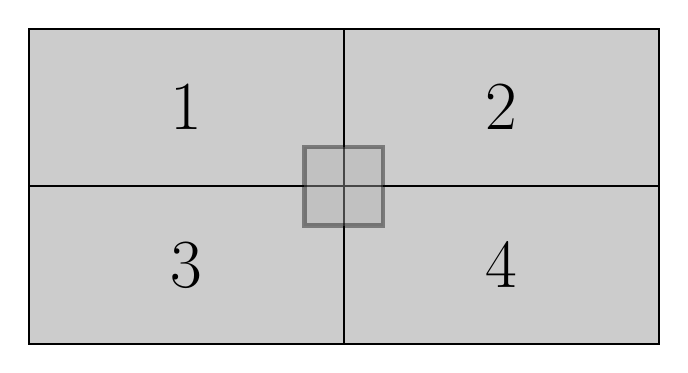
\begin{tikzpicture}
\draw[fill=black!20,thick] (0,0) rectangle node{\Huge$3$} (4,2);
\draw[fill=black!20,thick] (4,0) rectangle node{\Huge$4$} (8,2);
\draw[fill=black!20,thick] (0,2) rectangle node{\Huge$1$} (4,4);
\draw[fill=black!20,thick] (4,2) rectangle node{\Huge$2$} (8,4);
\draw[fill=black!30,ultra thick,opacity=0.4] (3.5,1.5) rectangle (4.5,2.5);
\end{tikzpicture}
\caption{Nomenclatura delle quattro aree che circondano il pilastro. Viene utilizzata nelle tabelle in cui vi è riportata l'estensione delle stesse e il relativo calcolo dello sforzo assiale}
\label{fig:NomenclaturaAree}
\end{figure}